%!TEX root=../../sbc-template.tex

Com a popularização das R-CNNs e o crescente interesse prático nas tarefas de detecção de objetos, em 2016 foi proposta a R-CNN YOLO (acrônimo para \emph{You Only Look Once}), a qual se propõe a realizar as tarefas de localização e classificação de múltiplos objetos em uma única etapa (\emph{single-shot}) \cite{Redmon:YOLOoriginal}. Essa R-CNN mostrou-se significativamente mais rápida para detecção do que os modelos anteriores do mesmo tipo disponíveis na literatura \cite{Michelucci:2019}.

Conforme ilustrado na Fig. \ref{fig:yolo_grid}, a abordagem de detecção de objetos por R-CNNs YOLO consiste nos seguintes passos: primeiramente há a divisão da imagem de entrada em uma grade de dimensões $S \times S$; em seguida, para cada célula, há uma verificação se há um objeto cujo centro é englobado pela mesma; para as células em que tal verificação foi afirmativa, calcula-se a quantidade $B$ de caixas delimitadores com seus respectivos coeficientes de confiança -- obtidos por meio da multiplicação da métrica IoU (do inglês, \emph{Intersection Over Union}) com a probabilidade da célula conter um certo objeto de uma dada classe -- refletindo numericamente o quão acurada está uma caixa delimitadora que contém o objeto; por fim, células adjacentes com alta confiança para um mesmo tipo de objeto são unificadas, culminando na previsão das coordenadas das caixas e seus respectivos rótulos \cite{Michelucci:2019}.

\begin{figure}[H]
    \centering
    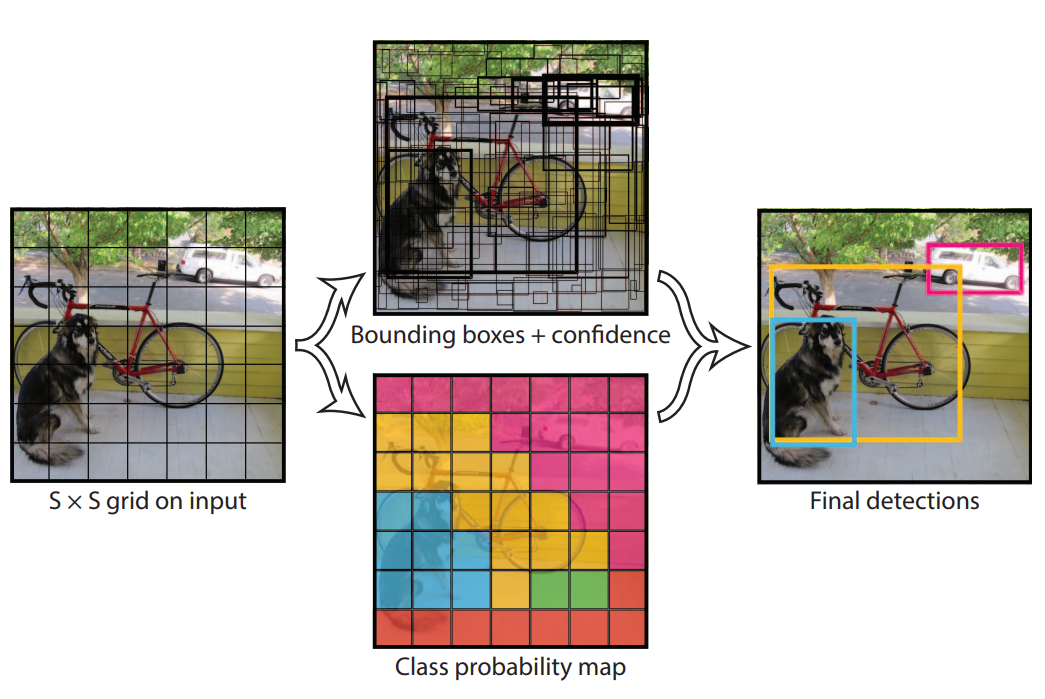
\includegraphics[width=0.70\textwidth]{img/yolo-approach}
    \caption{Abordagem da YOLO para detecção de objetos.
    Fonte: \cite{Redmon:YOLOoriginal}.}
    \label{fig:yolo_grid}
\end{figure}

A arquitetura utilizada na YOLOv1 (primeira versão) foi inspirada na CNN Inception pré-treinada com pesos oriundos da base de dados ImageNet \cite{ImageNet}. Esta arquitetura é constituída por $20$ camadas convolucionais seguidas por $2$ camadas totalmente conectadas. Ao invés de usar os módulos Inception originais, os autores da YOLO optaram por utilizar camadas de \emph{pooling} com filtros de dimensões $1\times 1$ para redução de dimensionalidade seguidos de camadas convolucionais com filtros $3 \times 3$, conforme ilustrado na Figura \ref{fig:yolo_arch}.

\begin{figure}[H]
    \centering
    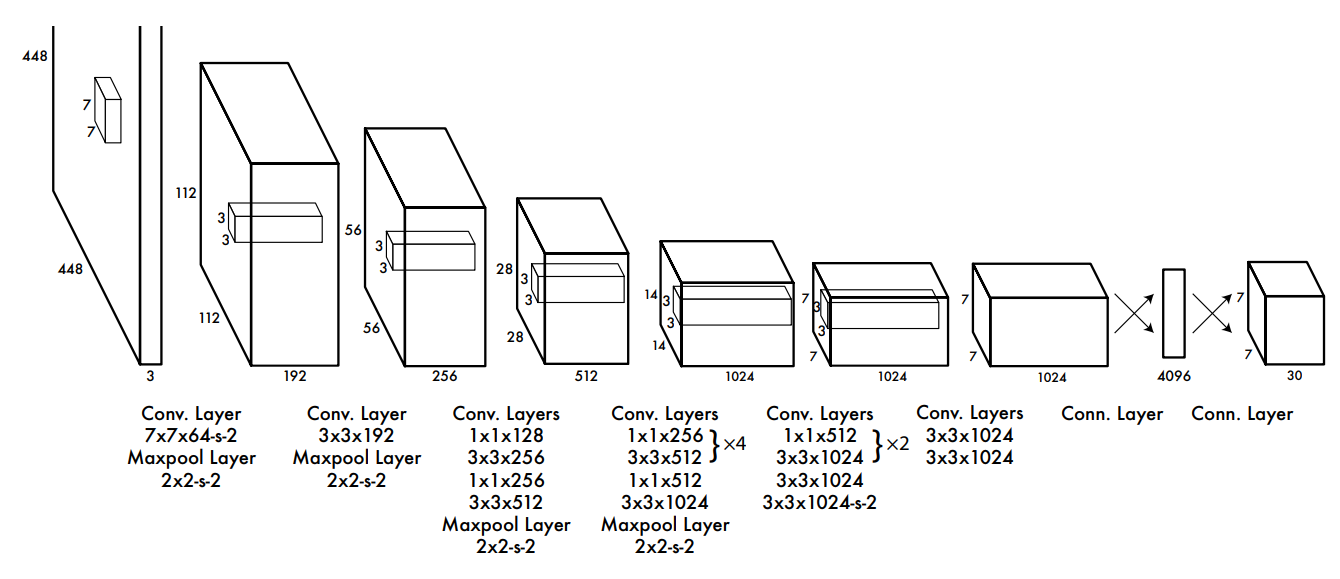
\includegraphics[width=\textwidth]{img/yolo-arquitetura}
    \caption{Arquitetura da CNN utilizada na primeira versão da YOLO.\\ Fonte: \cite{Redmon:YOLOoriginal}.}
    \label{fig:yolo_arch}
\end{figure}

% Seguir para Yolov4,  v5, v6 e v7.

Ao longos dos anos, novas técnicas e melhorias foram incorporadas em versões atualizadas de modelos da Família YOLO. Para a YOLOv4, por exemplo, utilizou-se o \emph{backbone} CSPDarkNet53, tornando-a duas vezes mais rápida que outras arquiteturas de referência na época do seu lançamento. Ainda, comparando com a sua versão anterior (YOLOv3) as métrica AP e FPS foram melhoradas em $\SI{10}{\percent}$ e $\SI{12}{\percent}$, respectivamente \cite{Bochkovski:YOLOv4}.

A YOLOv5 decorreu logo após a proposição da YOLOv4 tendo como maior diferença a implementação do \emph{framework} DarkNet de forma nativa com o Pytorch, o que facilitou drasticamente o treinamento e o \emph{deployment} desse modelo. A principal inovação da YOLOv5 em relação às suas antecessoras foi a introdução do \emph{Mosaic Augmentation}, uma técnica de regularização por meio do aumento artificial de dados que combina quatro imagens em quatro blocos de proporção aleatória. Conforme argumentam seus proponentes, a principal vantagem dessa inovação é a melhoria de desempenho na detecção de objetos pequenos. No sétimo \emph{release}, diferentes versões da YOLOv5 foram propostas para atender domínios específicos, citadas a seguir por ordem crescente de parâmetros e robustez: \emph{Nano}, \emph{Small}, \emph{Medium}, \emph{Large} e \emph{XLarge}. Os modelos mais simples visam aplicações embarcadas por serem mais leves, enquanto os mais complexos foram projetados para problemas mais difíceis, com imagens de maior dimensão, grande número de classes e tamanho de caixas delimitadoras bastante variados \cite{Jocher:YOLOv5}. A Figura \ref{fig:yolov5} ilustra o desempenho das diferentes versões da YOLOv5 perante a base de dados MS COCO \cite{Microsoft:COCO}, um \emph{benchmark} da literatura para detecção de objetos.

\begin{figure}[h!]
    \centering
    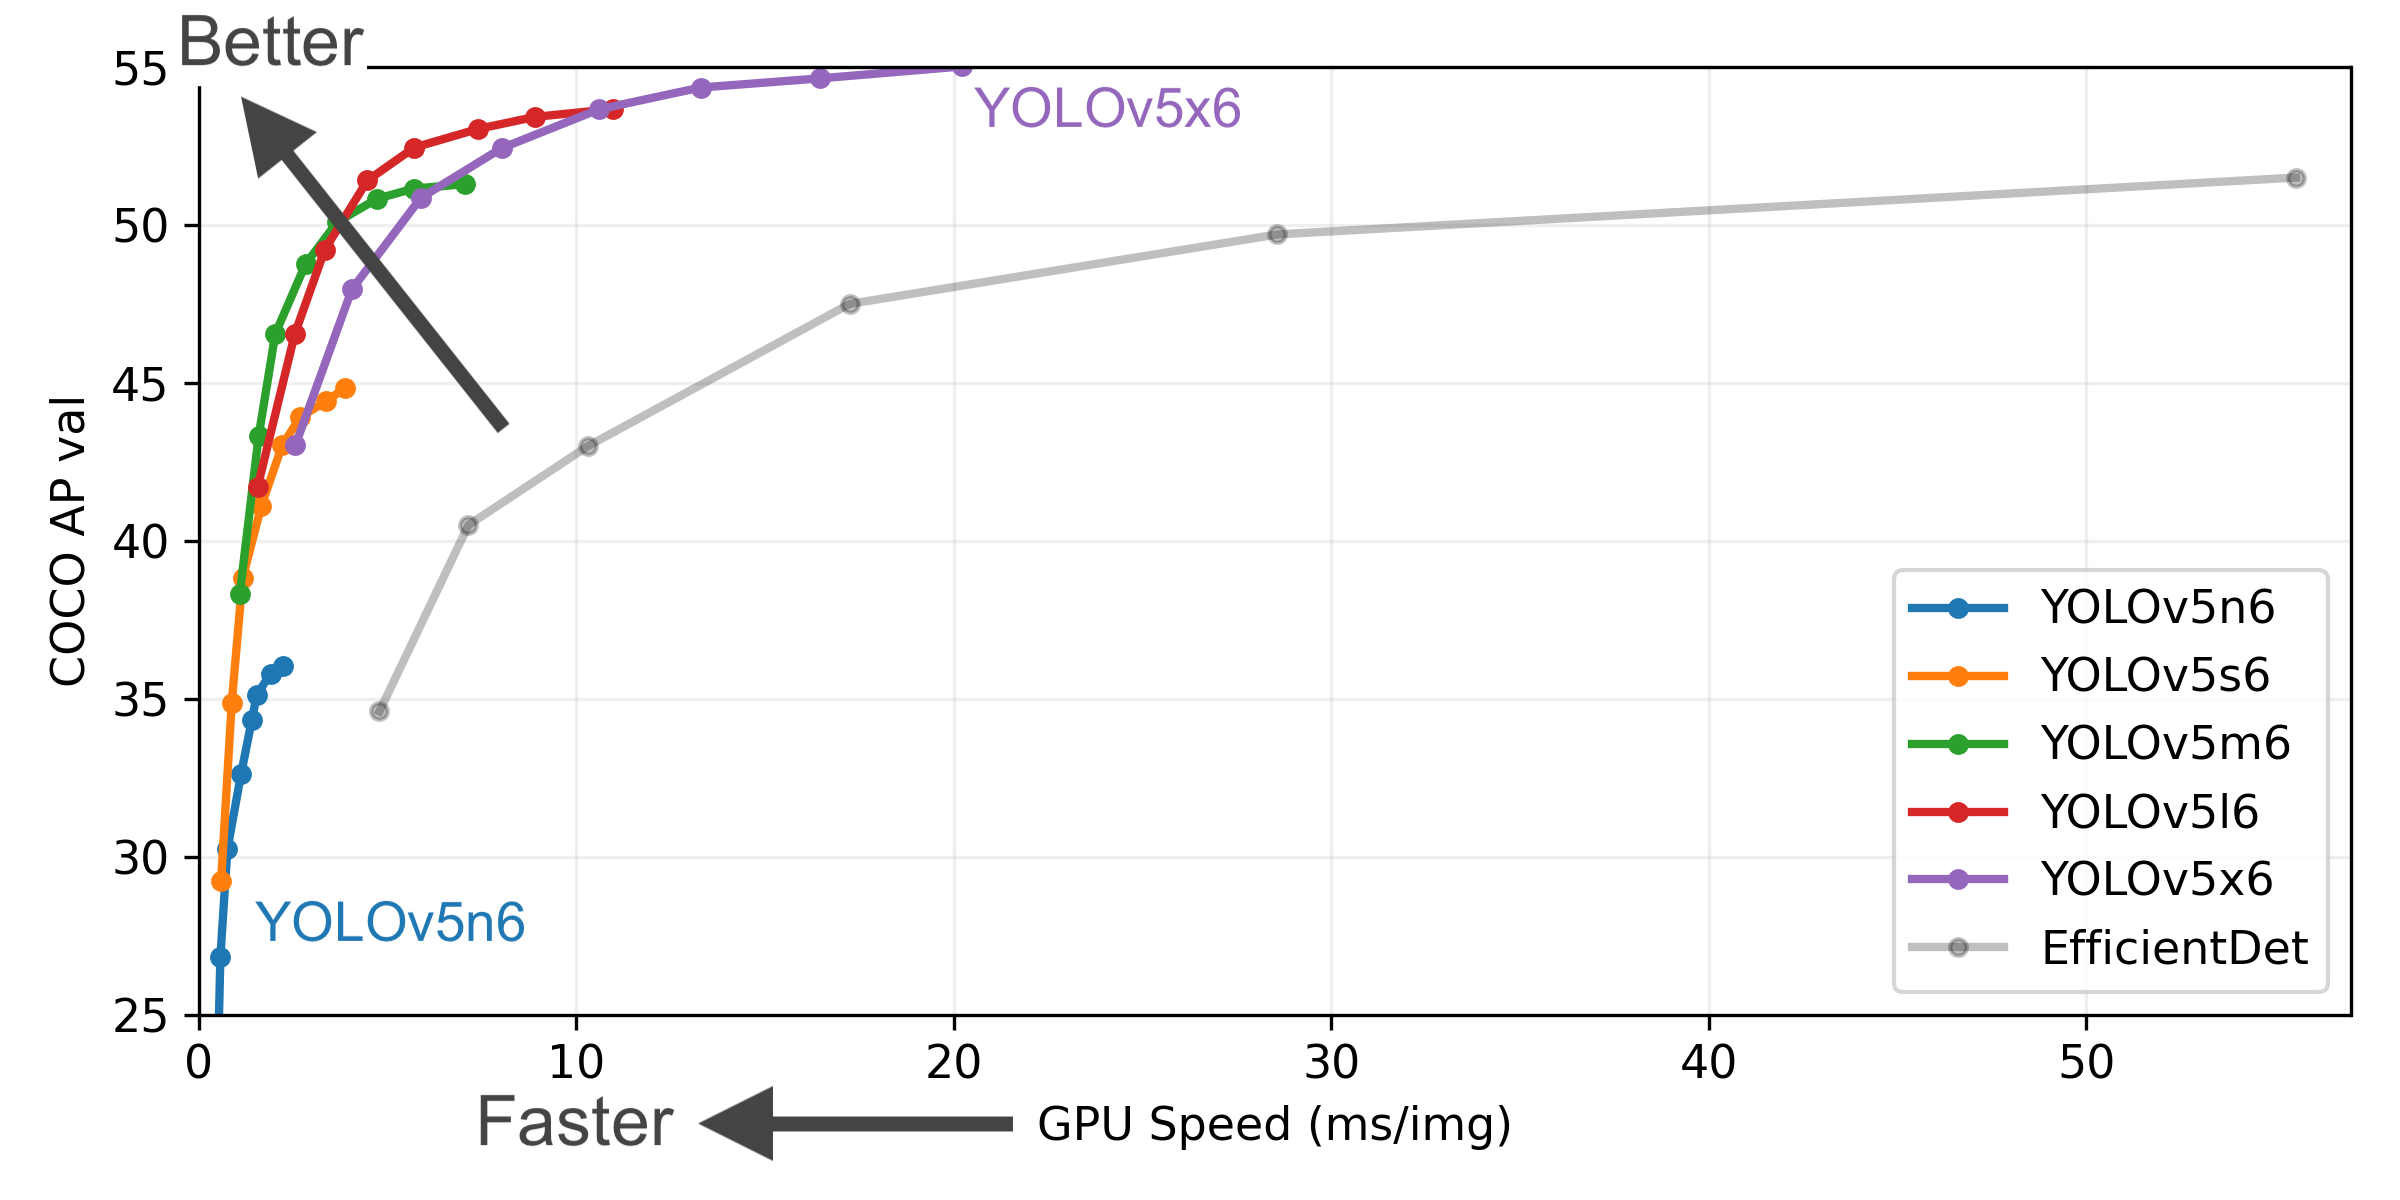
\includegraphics[width=0.8\textwidth]{./img/yolov5}
    \caption{Desempenho dos modelos YOLOv5 perante o MS COCO.\\ Fonte: \cite{Jocher:YOLOv5}.}
    \label{fig:yolov5}
\end{figure}

Outras versões da YOLO foram propostas por diferentes autores, mas nem todas se consolidaram perante a comunidade técnico-científica pois, apesar de apresentarem um bom desempenho no \emph{benchmark} MS COCO, não reproduziam tal eficiência em problemas de outros domínios. Ademais, era notável a dificuldade no treinamento em face da carência de documentação e de uma comunidade pequena de usuários. Como exemplo, cita-se o caso da YOLOv6 \cite{YOLOv6}.


A YOLOv7 deu continuidade ao aprimoramento dos modelos da Família YOLO ao incorporar um processo denominado reparametrização, com o intuito de diminuir o tamanho do modelo para \emph{deployment}, o que é especialmente útil para sistemas embarcados. Também faz uso de \emph{Feature Pyramid Networks} em sua arquitetura, as quais empilham camadas convolucionais e produzem previsões em diferentes escalas, colaborando para um melhor desempenho. Diferentemente das versões anteriores, propôs uma arquitetura padrão e uma estratégia de dimensionamento em escala para outras quantidades de parâmetros, sejam elas maiores ou menores \cite{yolov7}. A Figura \ref{fig:yolo-arch} apresenta uma análise comparativa entre os diferentes modelos da Família YOLO recém propostos na literatura perante o MS COCO.


\begin{figure}[h!]
    \centering
    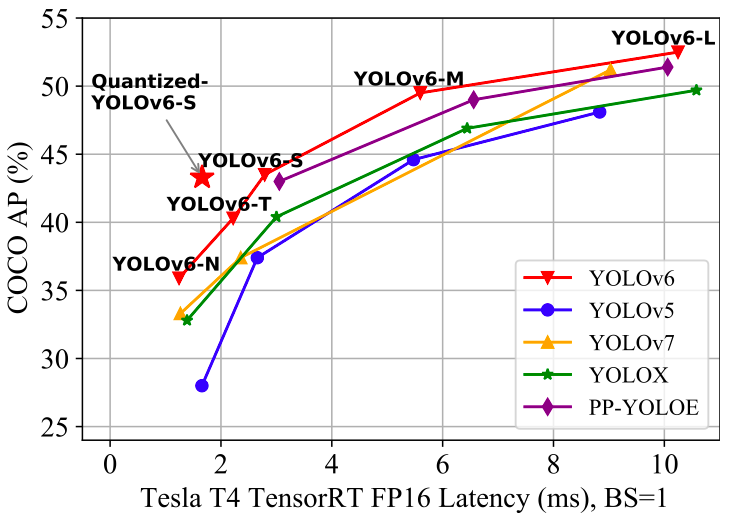
\includegraphics[width=0.75\textwidth]{img/yolo-latest-version}
    \caption{Comparação entre as últimas versões da YOLO propostas na literatura. O eixo vertical denota a eficiência do modelo e o eixo horizontal denota o tempo de treinamento.\\ Fonte: \cite{YOLOv6}.}
    \label{fig:yolo-arch}
\end{figure}